\section{Cluster Structures}

From the experimental results we can obtain two hints for the cluster
structure: the minimum size and the xenon content. In the following we will 
use these to construct representative cluster structures, for which we will 
simulate the ICD and ETMD spectra. At this point we put in a variety of
structures, in order to learn about general structure-spectrum relations
and therefore being able to
exclude some of them by comparison of
the ICD and ETMD spectra to the experimental ones.

In our previous study\cite{Fasshauer13} the ArXe clusters were assumed
to be large, having more than 1500 atoms. The model structures assumed
an fcc structure and not an icosahedral structure, which is energetically
favoured for small clusters.
Most estimated cluster sizes given in Table \ref{tab:cluster} are much smaller.
We use the estimated number of atoms for a pure Ar expansion as the lower limit for the actual cluster size and start our search for model structures from there.
%
%Additionally,
%the expectation value for the number of xenon atoms relies on a pure
%xenon gas. Since the xenon content in the mixed gas is much lower, also
%the number of xenon atoms can be expected to be by far less. We therefore
%start from the estimated number of atoms in the cluster after expansion
%of pure argon gas.
%We therefore rethink the possible cluster structures.
%Furthermore, the theoretical prediction did not match the experimental results.
%Since the spectra are strongly depending on the cluster structure as shown in
%\cite{fasshauer2014}, the underlying structure seems not to fit and hence
%we rethink the possible cluster structures.
%
For the smaller clusters measured,
these expectation values range from \unit[3--21]{Ar atoms}. 
The cluster sizes for expansion of a mixed gas are unknown, but
for xenon as the second component a larger size is expected compared to a
pure argon expansion, due to the higher polarizability
and hence larger cohesive energy of xenon. All clusters
contributing to the coincidence spectrum
contain at least one xenon atom, as otherwise decay by ICD or ETMD is energetically not allowed.

In a gas expansion a range of clusters sizes with different structures is produced. 
However, for small rare gas clusters consisting of less than approximately \unit[1000]{atoms} so-called \emph{islands of stability} were found.\cite{haberland}  
In mass spectra, clusters with mass numbers corresponding to icosahedral shapes had an abundance that was (slightly) enhanced over other sizes. 
We therefore started from icosahedral structures and constructed mixed cluster structures by substitution of individual atoms with one or the other kind (Ar or Xe), or added individual atoms close to the desired position within a given structure. 
After that, the cluster structures were optimized using the unified force
field implemented in the 
Avogadro programme (version 1.1.0) \cite{Avogadro,Hanwell12} to give local
minimum structures.
All cluster structures are listed in Table \ref{table:theo_gammas}.
%
\begin{figure}[ht]
 \centering
 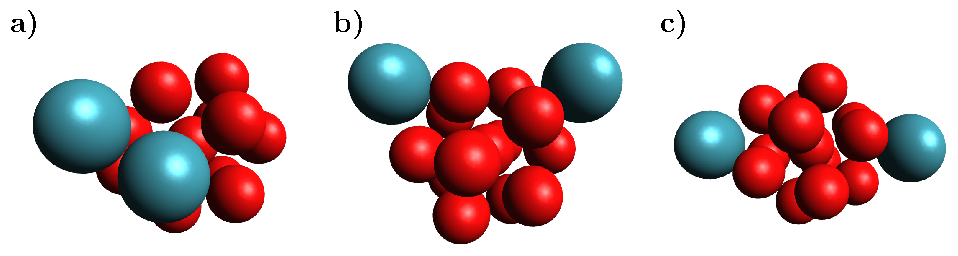
\includegraphics[width=8.5cm]{pics/cluster_2_overview.pdf}
 \caption{Cluster structures composed of 13 argon atoms and two additional xenon
          atoms on different surfaces of the argon icosahedron, varying in Xe-Xe distance:
          (a) closest possible, (b) middle, (c) furthest away. They refer to
          numbers 9--11 in Table \ref{table:theo_gammas}.}
 \label{figure:cluster_2_overview}
\end{figure}
%
\begin{figure}[h]
 \centering
 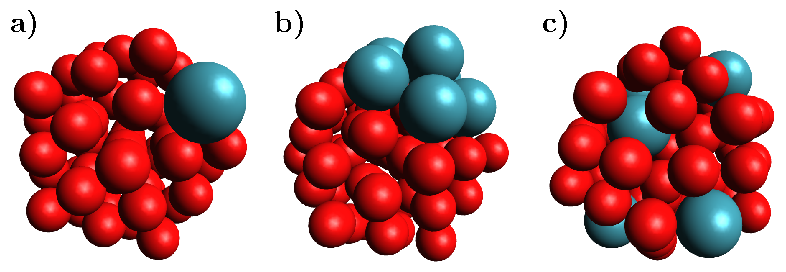
\includegraphics[width=8.5cm]{pics/cluster_3_overview.pdf}
 \caption{Cluster structures derived from a 55 atom icosahedral structure:
          (a) one xenon atom on the surface, (b) six xenon atoms inside a 55 atoms cluster,
          grouped on one side, (c) six xenon atoms distributed randomly
          in a 55 atoms cluster. They refer to numbers 12, 18 and 19
          in Table \ref{table:theo_gammas}.}
 \label{figure:cluster_3_overview}
\end{figure}

As discussed in the introduction, the small clusters will likely
deviate from a core-shell structure with a xenon core surrounded
by argon shells, as observed for large clusters.\cite{tchaplyguinearxe,Vach_1999} We therefore start from
argon clusters of 13 or 55 atoms, and modify them in one of the following
ways:
%
\begin{itemize}
 \item add one xenon atom on top of a surface / edge / vertex of
       the argon core, with an example shown in
       Figure \ref{figure:cluster_3_overview}a
       (one additional xenon atom
       on top of a surface of a \unit[55]{atom} argon core)
       (Table \ref{table:theo_gammas}, \#6--8, \#12--14),
 \item substitute one argon atom in a surface / edge / vertex position
       (Table \ref{table:theo_gammas}, \#15--16),
 \item substitute one or two argon atoms in the core of the argon cluster
       by xenon atom(s) for the simulation of the core-shell structures
       (Table \ref{table:theo_gammas}, \#1--3),
 \item add two xenon atoms on top of surfaces of a 13 atoms argon core
       in different relative positions (see Figure
       \ref{figure:cluster_2_overview}),
       in order to achieve a xenon content in the cluster close to the
       measured one (see below)
       (Table \ref{table:theo_gammas}, \#9--11),
 \item substitute six argon atoms of a 55 atoms argon cluster by xenon
       atoms either grouping them or distributing them througout the cluster
       (see Figure \ref{figure:cluster_3_overview}b and c) in order to
       achieve a xenon content in the cluster close to the measured one
       (Table \ref{table:theo_gammas}, \#18--19).
\end{itemize}

These structures were then optimized using force field methods.
%
Furthermore, for comparison with the largest measured ArXe clusters, we constructed also larger core-shell structures (Table \ref{table:theo_gammas}, \#4--5).
